\documentclass{beamer}
\usetheme{Berkeley}
%\usecolortheme{dove}
\usepackage{graphicx}
\usepackage{algpseudocode}
\usepackage[font={footnotesize}]{caption}
\newcommand{\A}{\texttt{A}}
\newcommand{\G}{\texttt{G}}
\newcommand{\U}{\texttt{U}}
\newcommand{\C}{\texttt{C}}
\newcommand{\klf}{\textsc{k-Local Folding} }
\newcommand{\rf}{\textsc{DP Folding} }

\title{A Local Alignment Approach to RNA folding}
\author{Ben Chugg, Coulter Beeson, Kenny Drabble, Jeff Jeyachandren}
\institute{\textsc{The University of British Columbia}}
\date{April 6,2017}

\begin{document}
\begin{frame}
\titlepage
\end{frame}


\begin{frame}
\section*{Background}
\frametitle{RNA Folding}
RNA consists of the four base pairs Adenine (\A), Guanine (\G) , Cytosine (\C) and Uracil (\U). These base pairs of RNA pair in a complementary fashion: Adenine to Uracil ($\A-\U$) and Cytosine to Guanine ($\C-\G$). \\

Unlike DNA for which we are concerned with optimally aligning two strands, for RNA we are concerned with how the strand folds with itself. 

\begin{figure}
\centering
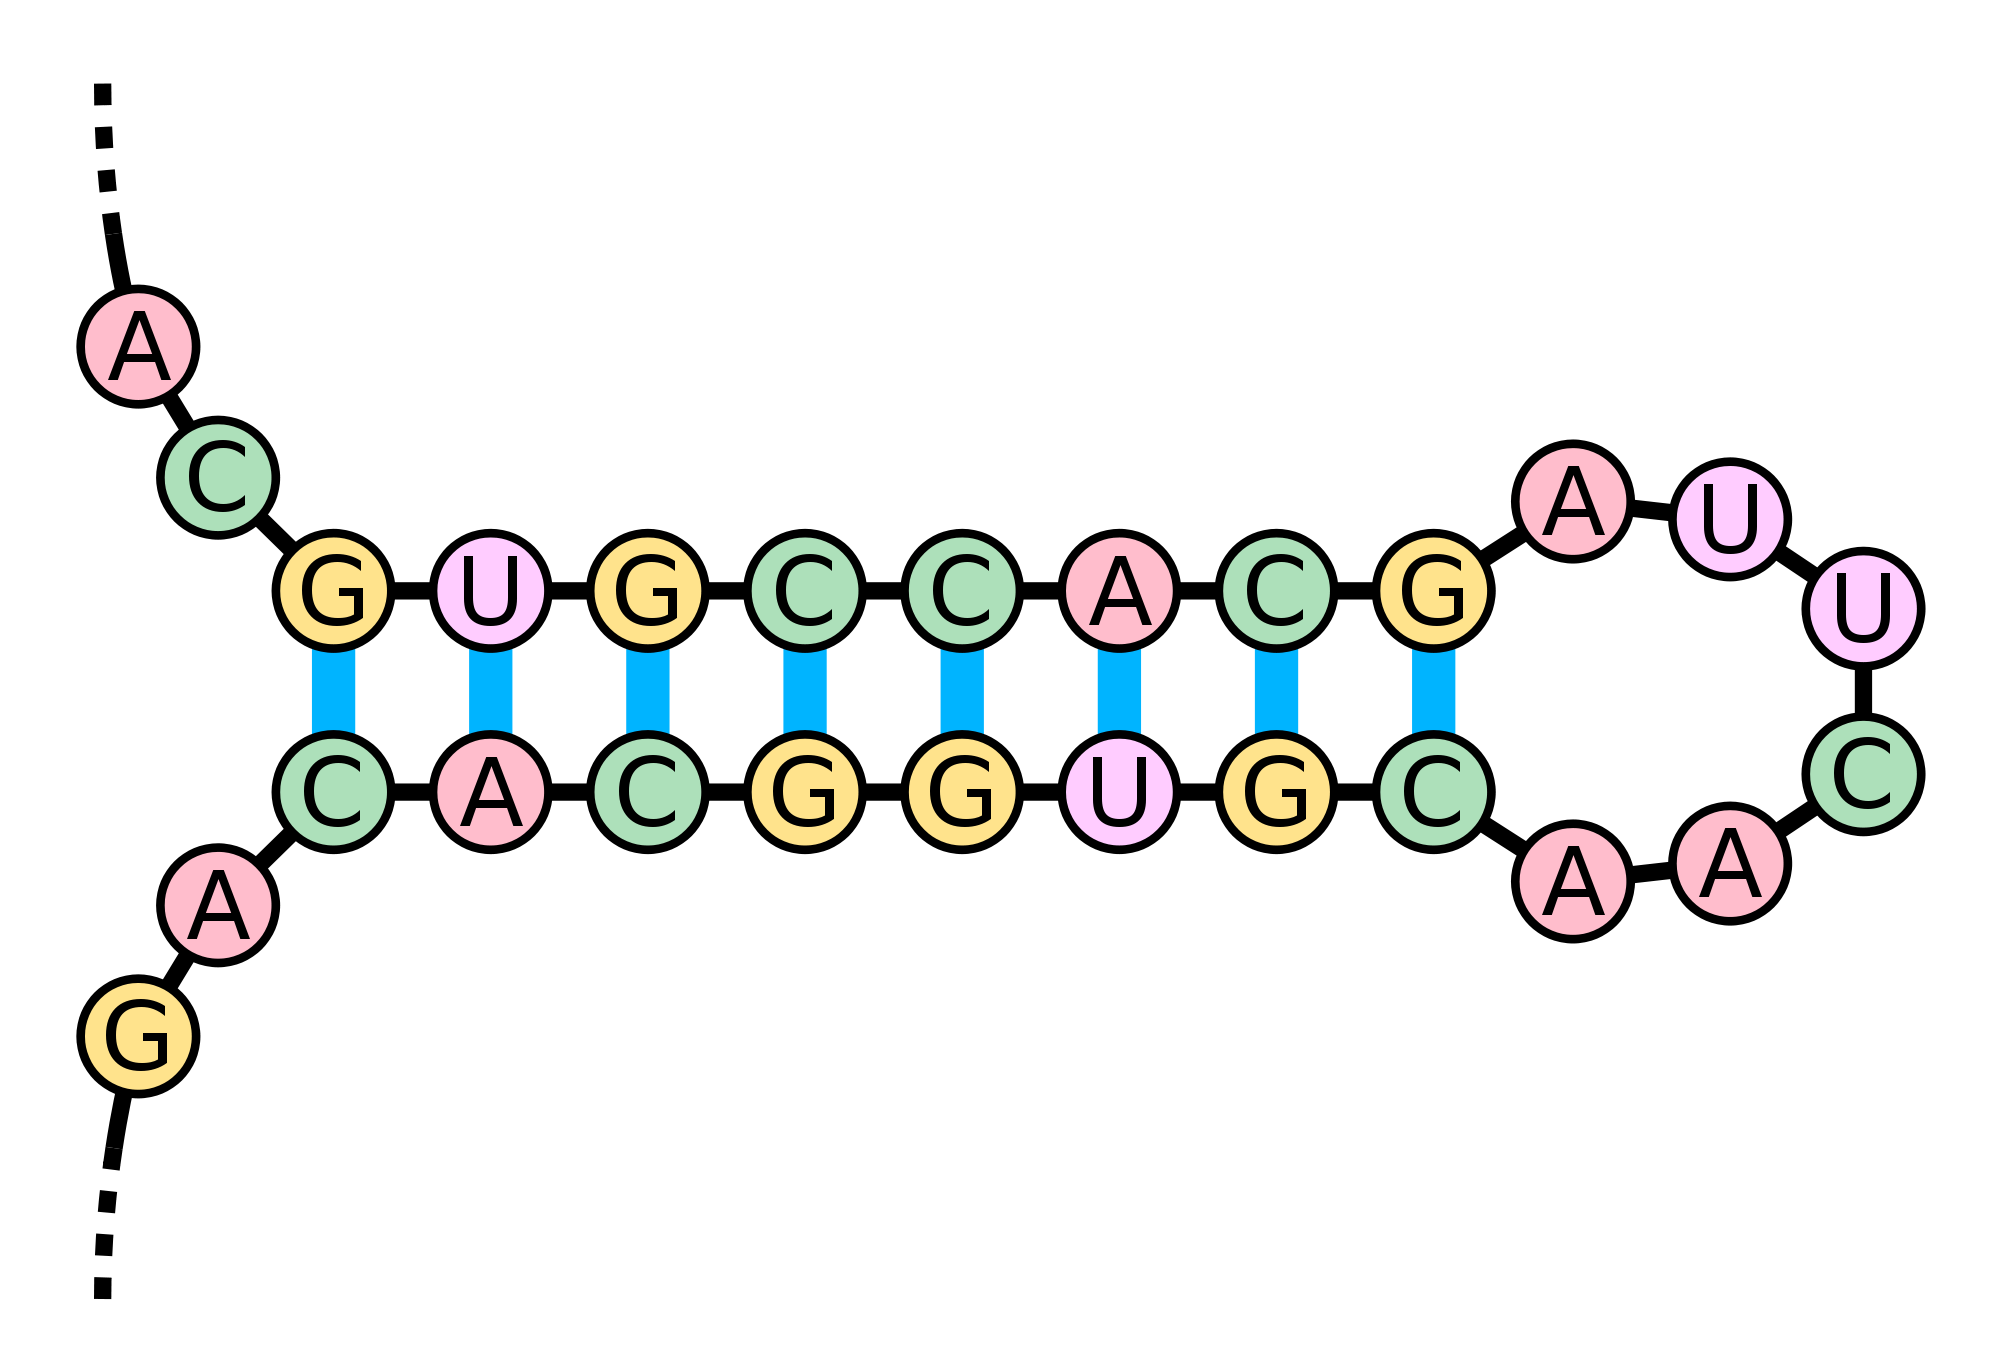
\includegraphics[scale=0.07]{images/hairpin_loop.png}
\vspace{-0.2cm}
\caption{Source: \url{http://rosalind.info/problems/pmch/}}
\end{figure}
\end{frame}

\begin{frame}
\frametitle{RNA Folding}
There are several frameworks with which we can model RNA folding. We will use the Energy Minimization Model. \\

In this model, matches are scored as $+1$ and non-matches as 0. This lends itself to a dynamic programming approach. Let $r=r_1,\ldots,r_n$ be a strand of RNA, where $r_i\in\{\A,\C,\G,\U\}$ and let $S(i,j)$ denote the optimal score of folding the subsequence $s_i,s_{i+1}\ldots s_j\subset s$. Then, 
\[S(i,j)=\max\begin{cases}
S(i+1,j-1)+1,&\text{if }i,j\text{ base pair}\\
S(i+1,j),\\
S(i,j-1),\\
\displaystyle \max_{i<k<j}\{S(i,k)+S(k+1,j)\},&\text{bifurcation}.
\end{cases}\]
\end{frame}

\begin{frame}
\frametitle{RNA Folding}
Problems with the Energy Minimization Model:
\begin{enumerate}
\item Simplicity
\item Does not capture pseudo-knots
\end{enumerate}

\begin{definition}
A strand $r=r_1,\ldots,r_n$ is said to contain a pseudo knot if there exist indicies $i_1<i_3<i_2$ and $j_1<j_3<j_2$ such that $r_{i_1},\ldots,r_{j_1}$ is aligned with $r_{i_2},\ldots,r_{j_2}$  and $r_{i_3},\ldots,r_{j_4}$ is paired with a subsequence outside the interval $r_{i_1},\ldots,r_{j_2}$. 
\end{definition}
\end{frame}

\begin{frame}
\frametitle{RNA Folding}
\begin{figure}
\centering
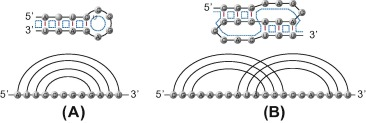
\includegraphics[scale=0.8]{images/pseudoknot.jpg}
\caption{Source: \url{http://www.sciencedirect.com/science/article/pii/S0025556413001788}}
\end{figure}

We will call this typical RNA folding algoritm \rf. 

\end{frame}

\begin{frame}
\frametitle{k-Local Folding}
\section*{Our Approach}
Idea: Subsequences of an RNA strand which are (near) palindromes of each other are likely to be a good match. \\

Formally, we define an algorithm \klf which takes as input an RNA strand $r$ and a parameter $k$, runs a local alignment algorithm on the strand to find $k$ high scoring --- and disjoint --- palindromic regions of $r$. It then passes the remaining unpaired regions to \rf to be folded as usual. 

\begin{algorithmic}
\Function{k-Local Folding}{$r,k$}
\State Call Smith Waterman on $r$ $k$ times 
\EndFunction
\end{algorithmic}

\end{frame}
\end{document}